\documentclass[conference]{IEEEtran}
\IEEEoverridecommandlockouts

% ---------------------------------------------------------------
% Packages
% ---------------------------------------------------------------
\usepackage{cite}
\usepackage{amsmath,amssymb,amsfonts}
\usepackage{algorithmic}
\usepackage{graphicx}
\usepackage{textcomp}
\usepackage{xcolor}
\usepackage{booktabs}
\usepackage{multirow}
\usepackage{tabularx}
\usepackage{url}
\usepackage{natbib}
\usepackage{hyperref}
\usepackage{microtype}
\usepackage{array}
\usepackage[T1]{fontenc}

\hypersetup{
    colorlinks=true,
    linkcolor=blue,
    citecolor=blue,
    urlcolor=blue
}

\def\BibTeX{{\rm B\kern-.05em{\sc i\kern-.025em b}\kern-.08em
    T\kern-.1667em\lower.7ex\hbox{E}\kern-.125emX}}

% ---------------------------------------------------------------
\begin{document}

\title{Hierarchical Multi-Agent Deep Reinforcement Learning\\
for Urban Traffic Signal Control at Scale}

\author{
\IEEEauthorblockN{Satya Srinivas Paladugu}
\IEEEauthorblockA{Department of Artificial Intelligence\\Amrita Vishwa Vidyapeetham\\Bengaluru, India\\bl.ai.u4aid24063@bl.students.amrita.edu}
\and
\IEEEauthorblockN{Roydon Vilber Rodrigues}
\IEEEauthorblockA{Department of Artificial Intelligence\\Amrita Vishwa Vidyapeetham\\Bengaluru, India\\bl.ai.u4aid24059@bl.students.amrita.edu}
\and
\IEEEauthorblockN{Prithvi S}
\IEEEauthorblockA{Department of Artificial Intelligence\\Amrita Vishwa Vidyapeetham\\Bengaluru, India\\bl.ai.u4aid24076@bl.students.amrita.edu}
\and
\IEEEauthorblockN{Dr. Manju  Venugopalan}
\IEEEauthorblockA{Department of Artificial Intelligence\\Amrita Vishwa Vidyapeetham\\Bengaluru, Vidyapeetham\\Bengaluru, India\\v\_manju@blr.amrita.edu}
}

\maketitle

% ---------------------------------------------------------------
%  ABSTRACT
% ---------------------------------------------------------------
\begin{abstract}
Urban traffic congestion in dense metropolitan regions such as Bengaluru, India,
presents a control problem that flat or single-intersection approaches cannot
adequately address. This paper introduces a three-tier Hierarchical Multi-Agent
Reinforcement Learning (HMRL) framework for city-scale adaptive traffic signal
control. The architecture operates across a Ward Layer (L1), which manages
individual intersections using Proximal Policy Optimization (PPO) and Deep
Q-Networks (DQN); an Area Layer (L2), which coordinates adjacent wards through
a Spatio-Temporal Graph Convolutional Network (STGCN); and a City Layer (L3),
which resolves macro-level origin-destination flow using NetworkX-based
min-cost graph optimization.

Simulation environments are built from real OpenStreetMap data for 16 wards
across four areas in the South Bengaluru corridor---HSR Layout, BTM Layout, BTM
Layout Extension, and Jayanagar---processed through the SUMO microscopic traffic
simulator. Vehicle heterogeneity is explicitly modeled: seven distinct vehicle
classes (including BMTC buses, aggressive drivers, ambulances, and government
convoys) operate under six scenario configurations spanning baseline, peak
congestion, breakdown cascade, ambulance emergency, VIP convoy, and full chaos
conditions. A zone-aware reward function penalizes queue length, cumulative
delay, and wait time while rewarding throughput and speed, with modulations
per zone type (commercial, arterial, hospital-sensitive, IT corridor).

Ablation studies compare fixed-time baselines, ward-only RL, ward-plus-area
coordination, and the full three-layer hierarchy across all scenarios.
[PLACEHOLDER: Results summary to be inserted after training runs complete.]
The framework demonstrates that hierarchical decomposition directly addresses
the curse of dimensionality that limits centralized city-wide controllers,
and that STGCN-based area coordination materially improves green-wave
propagation compared to independent per-ward agents.
\end{abstract}

\begin{IEEEkeywords}
hierarchical reinforcement learning, multi-agent systems, traffic signal control,
spatio-temporal graph convolutional network, SUMO, Bengaluru, proximal policy
optimization, deep Q-network, urban mobility
\end{IEEEkeywords}

% ---------------------------------------------------------------
%  I. INTRODUCTION
% ---------------------------------------------------------------
\section{Introduction}

Traffic signal control in large cities is not a single-intersection problem.
A jam at one junction backs up into the next, which changes optimal phase
timings two blocks away, which shifts origin-destination pressure on arterials
across an entire district. Any controller that ignores this spatial coupling
will locally optimize while globally failing.

Bengaluru's road network illustrates this at scale. The city's South Corridor---
covering areas such as HSR Layout, BTM Layout, and Jayanagar---connects dense
residential zones to major IT corridors. Morning peak loads can reach 3.5$\times$
baseline vehicle counts, with simultaneous ambulance dispatch, government convoys,
and cascading breakdowns regularly co-occurring. Fixed-time signals, which still
control the majority of intersections in Indian cities, cannot adapt to any of
these conditions.

The dominant approach in recent literature is single-intersection deep
reinforcement learning, with DQN and PPO variants applied to synthetic or
simplified grid networks \cite{shalaby2021intelligent, acm2021drl}. A parallel
thread applies multi-agent RL (MARL) to groups of intersections, but most MARL
formulations suffer from non-stationarity: each agent's environment changes as
other agents learn, destabilizing training \cite{marl2025sciencedirect}.
Graph-based representations have been proposed to address spatial coupling
\cite{graphbased2023arxiv}, and hierarchical decompositions have shown promise
in reducing the action space each individual agent must cover
\cite{hier2024naturereports, hier2024hierarchical}.

What remains rare is a framework that combines all three components---ward-level
RL, graph-based mesoscopic coordination, and city-level macro-flow
optimization---inside a realistic heterogeneous simulation of an Indian urban
road network, with explicit vehicle-class diversity and scenario stress testing.

This paper makes the following contributions:

\begin{enumerate}
    \item A three-tier HMRL architecture (L1 Ward, L2 Area, L3 City) with
    explicit timescale separation (30\,s / 60\,s / 120\,s tick intervals),
    enabling each layer to operate at the time resolution appropriate to its
    spatial scope.

    \item A Spatio-Temporal Graph Convolutional Network (STGCN) at the area
    layer that learns to predict ward-level congestion pressure 30 seconds
    ahead, providing anticipatory bias signals to ward agents rather than
    reactive corrections.

    \item A zone-aware, multi-component reward function with per-zone-type
    weight modulation (arterial, commercial, residential, hospital-sensitive,
    IT corridor, bottleneck) and explicit ambulance and incident sub-components.

    \item A simulation pipeline built from real Bengaluru OpenStreetMap data
    with seven vehicle classes, six stress scenarios, and realistic breakdown
    and convoy injection, validated against SUMO's microscopic physics engine.

    \item Ablation studies isolating the contribution of each hierarchy layer
    across six scenario types, enabling direct measurement of the area GNN's
    coordination value.
\end{enumerate}

The remainder of the paper is structured as follows. Section~\ref{sec:related}
reviews related work. Section~\ref{sec:system} describes the simulation
environment and data pipeline. Section~\ref{sec:rl} presents the RL foundations.
Section~\ref{sec:arch} details the three-layer hierarchy. Section~\ref{sec:eval}
describes the evaluation methodology and presents results.
Section~\ref{sec:conclusion} concludes.

% ---------------------------------------------------------------
%  II. RELATED WORK
% ---------------------------------------------------------------
\section{Related Work}
\label{sec:related}

\subsection{Single-Intersection Deep RL}

The foundational line of work frames each intersection as a separate MDP,
training DQN agents on queue length and phase observations
\cite{acm2021drl, shalaby2021intelligent}. These approaches achieve clear
improvements over fixed-time and Webster-actuated baselines on synthetic
grids, but do not generalize to corridor-scale coordination: a locally
optimal phase at one junction may increase upstream queue pressure on its
neighbor.

\subsection{Multi-Agent Traffic Control}

Multi-agent extensions apply independent learners to multiple intersections
simultaneously. \citeauthor{marl2025sciencedirect} \cite{marl2025sciencedirect}
survey the stability challenges in MARL traffic settings, noting that
non-stationarity makes convergence guarantees difficult when agents share
a road network. Cooperative reward shaping and shared replay buffers partially
mitigate this but do not resolve the fundamental curse of dimensionality
as network size grows.

Emergency vehicle priority adds a further constraint. \citeauthor{multiagent2022emergency}
\cite{multiagent2022emergency} propose multi-agent coordination for ambulance
corridor clearance, demonstrating that without explicit priority actions,
standard RL agents learn to locally minimize delay while blocking emergency
routes. Our architecture addresses this through explicit ambulance and incident
sub-components in the reward function and a dedicated CLEAR\_AMBULANCE\_PATH
action at the ward layer.

\subsection{Hierarchical Reinforcement Learning}

Hierarchical RL for traffic control has been explored in several recent
works. \citeauthor{hier2024naturereports} \cite{hier2024naturereports}
demonstrate improved convergence stability in multi-intersection settings
by decomposing the policy into a high-level goal selector and a low-level
phase executor. \citeauthor{hier2024hierarchical} \cite{hier2024hierarchical}
apply a two-level hierarchy with predictable cycle planning, reducing the
variance in lower-level policies. \citeauthor{hierarchical_megacity} \cite{hierarchical_megacity}
scale hierarchical RL to megacity road networks, showing that flat approaches
become computationally intractable beyond a few hundred intersections.

Our work extends these by adding a third city-level layer with graph-theoretic
flow optimization, and by grounding the simulation in real OSM map data for
an Indian urban corridor.

\subsection{Graph Neural Networks for Traffic Forecasting}

STGCN for traffic forecasting was introduced by \citeauthor{stgcn_ieee} \cite{stgcn_ieee},
combining graph convolutions for spatial dependency modeling with
gated recurrent units for temporal dynamics. This architecture was
subsequently applied to multi-graph road networks by \citeauthor{ddpgcn2021}
\cite{ddpgcn2021}, who demonstrated that capturing both speed and flow
on separate graph channels improves prediction accuracy over single-graph
methods. \citeauthor{gnn_traffic_bs} \cite{gnn_traffic_bs} extend these results
to Bengaluru-specific road topology, confirming that GNN-based forecasters
outperform classical time-series models on Indian arterial networks.

In our architecture, the STGCN operates at the area layer as a congestion
pressure forecaster---not a standalone predictor---feeding anticipatory
bias signals into the ward-level RL reward and observation.

\subsection{Real-World Traffic Simulation}

\citeauthor{aitraffic_sumo} \cite{aitraffic_sumo} validate SUMO as a
microscopic simulator for RL-based traffic control research, establishing
that TraCI-based policy injection produces results transferable to
vehicle-level dynamics. \citeauthor{sustainability_marl} \cite{sustainability_marl}
apply sustainability objectives to hierarchical MARL, using SUMO environments
with heterogeneous vehicle mixes to evaluate emissions alongside delay.
\citeauthor{deeprl_navigation} \cite{deeprl_navigation} apply deep RL
to real-time vehicle navigation, demonstrating that learned policies
can generalize across unseen road conditions when trained on diverse
scenario distributions.

% ---------------------------------------------------------------
%  III. SIMULATION ENVIRONMENT
% ---------------------------------------------------------------
\section{Simulation Environment and Data Pipeline}
\label{sec:system}

\subsection{SUMO as the Microscopic Simulator}

SUMO (Simulation of Urban MObility) \cite{aitraffic_sumo} operates at the
vehicle level: every car, bus, bike, and truck has its own route, speed,
and car-following dynamics. This matters for our problem because aggregate
models cannot capture the blocking behavior of a stalled truck on a two-lane
arterial or the gap-opening dynamics when an ambulance activates its siren.

The SUMO simulation accepts three primary inputs: a road network file
(\texttt{*.net.xml}), a route file (\texttt{*.rou.xml}), and a master
configuration file (\texttt{*.sumocfg}). External Python code connects via
TraCI (Traffic Control Interface), a TCP-based API that allows the
reinforcement learning layer to read sensor states and inject control commands
at each simulation step.

\begin{figure}[!t]
\centering
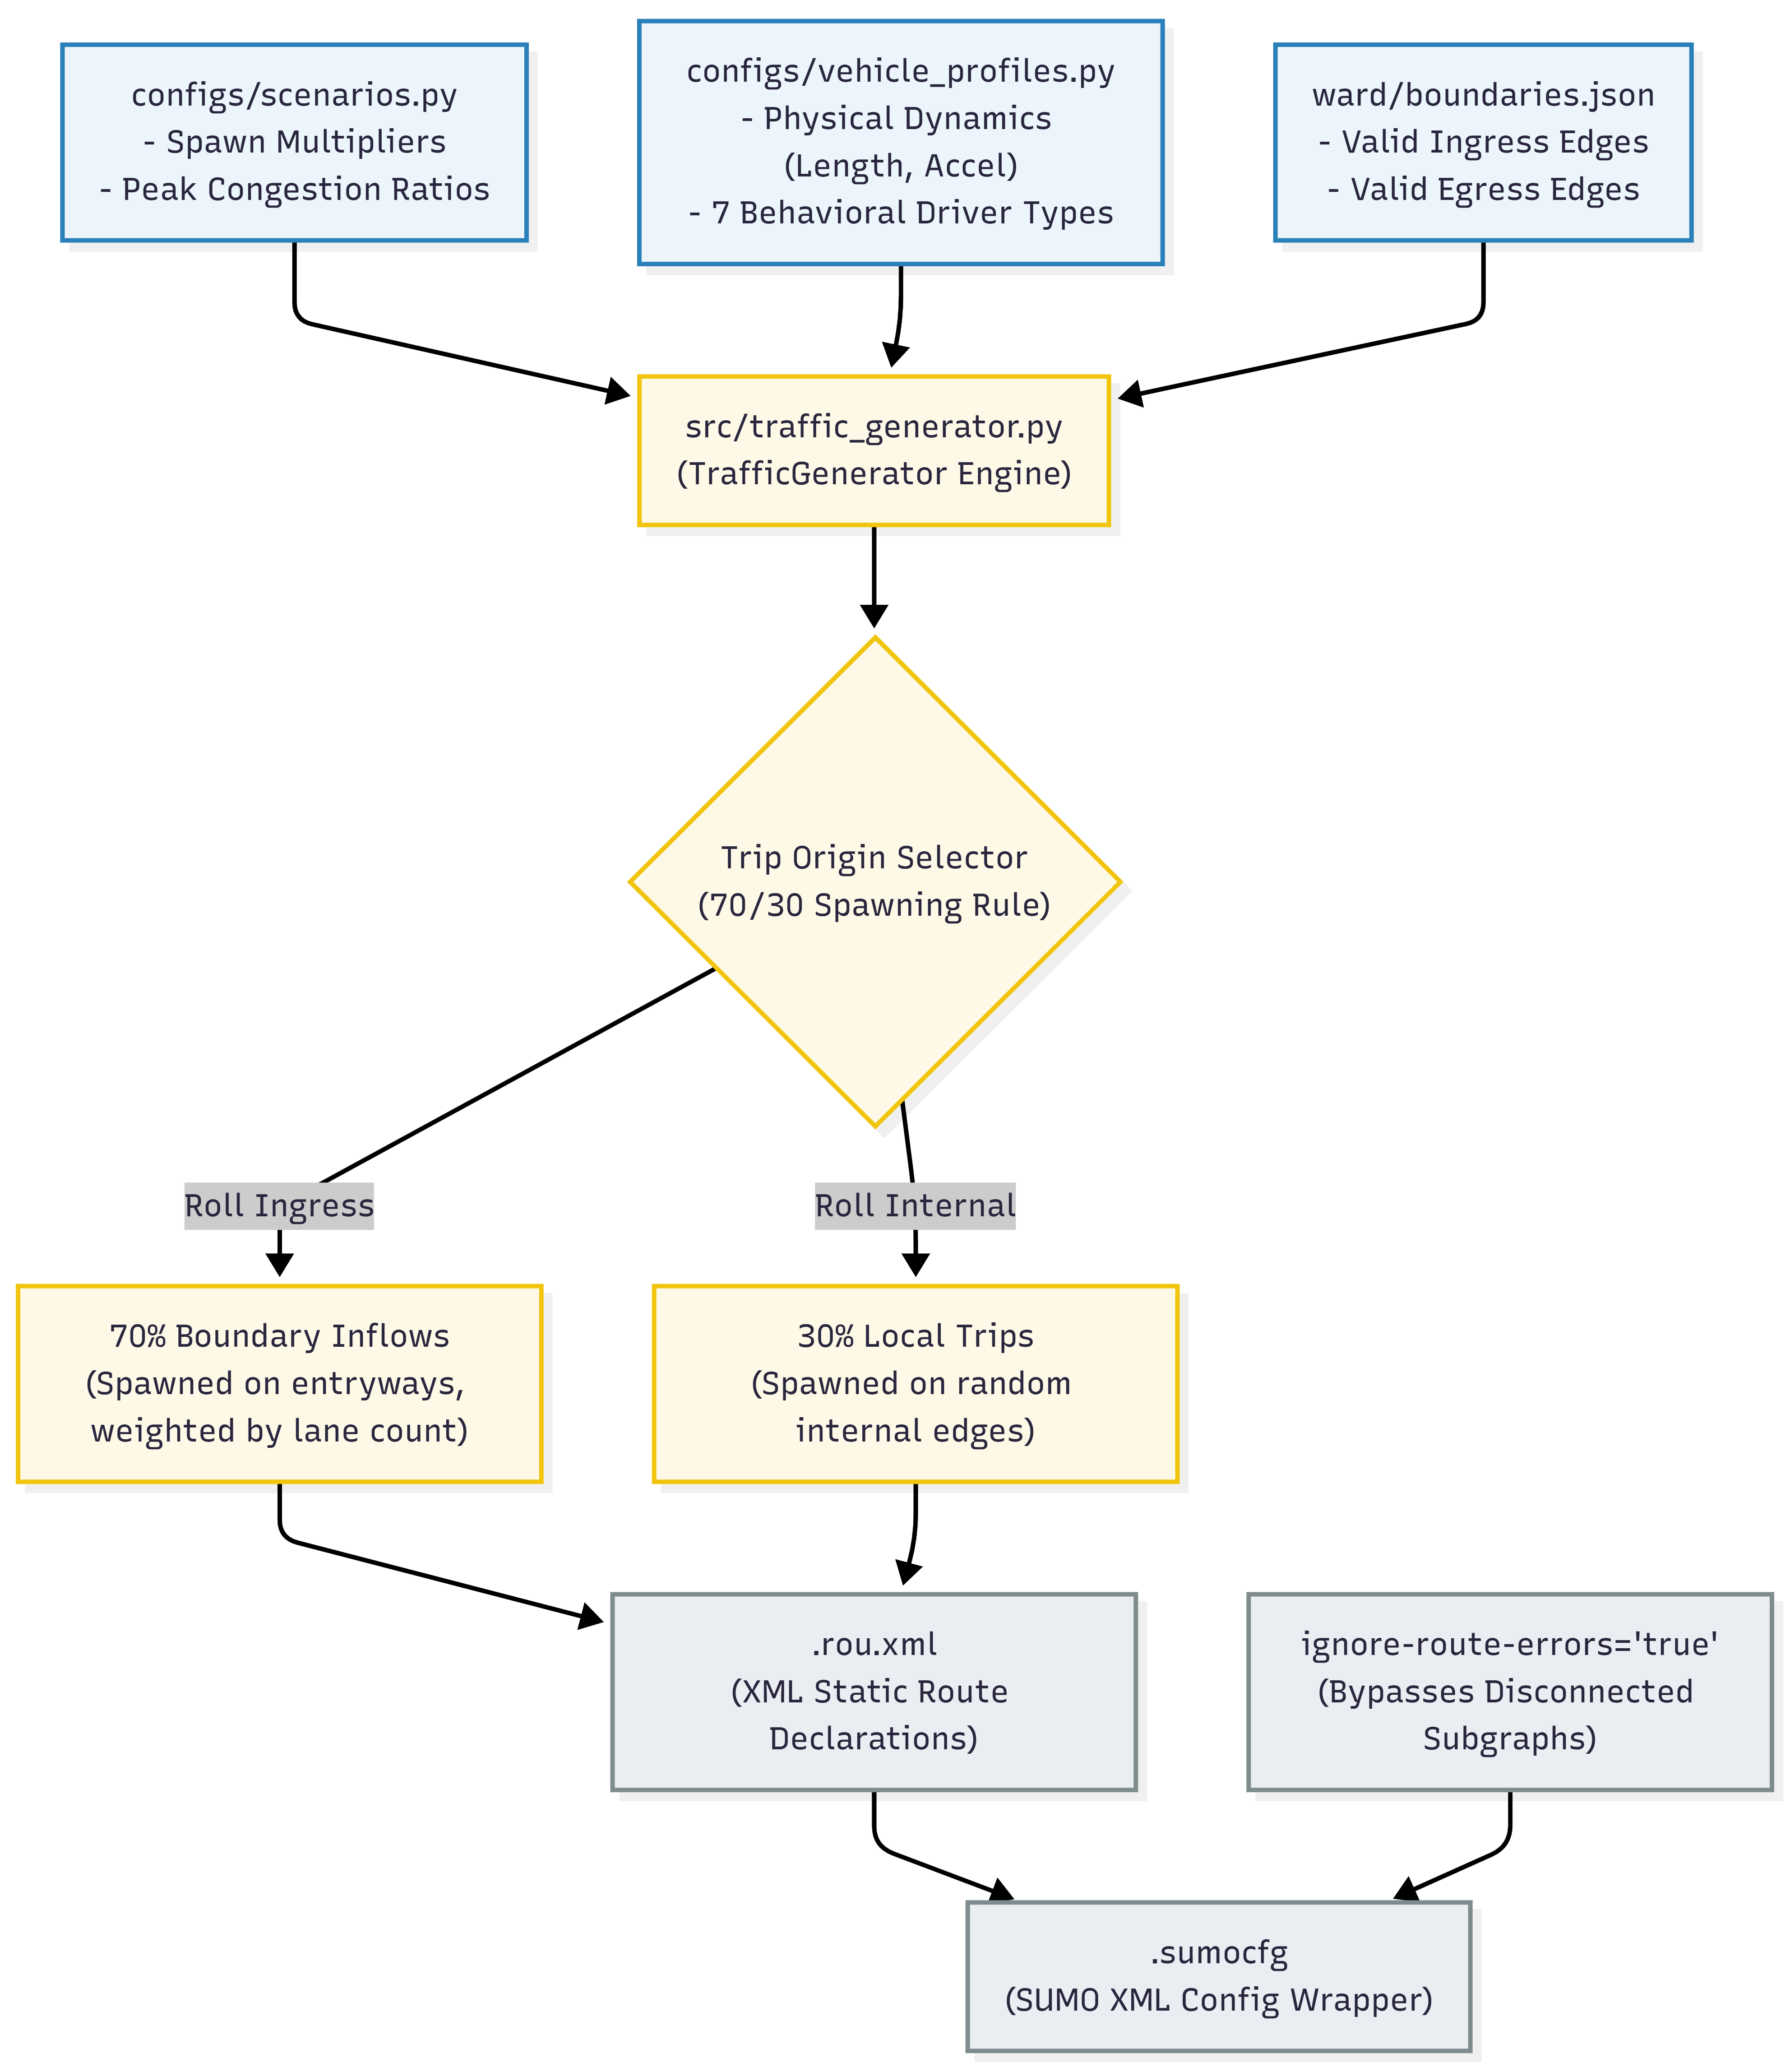
\includegraphics[width=\linewidth]{diagrams/RouteGeneration.png}
\caption{Traffic Demand and Route Generation Pipeline}
\label{fig:route_generation}
\end{figure}

\subsection{Map Acquisition and Processing Pipeline}

Rather than using synthetic grid networks, we build simulation environments
from real Bengaluru road geometry. The pipeline proceeds in three stages.

\textbf{Stage 1: OSM Extraction.}
Ward boundaries for Bengaluru's BBMP administrative divisions are resolved
through the Overpass API using ward-boundary queries at \texttt{admin\_level=10}.
For each ward, highway ways within the administrative polygon are extracted
as raw \texttt{*.osm} files.

\textbf{Stage 2: Network Compilation.}
Raw OSM files are processed through SUMO's \texttt{netconvert} utility with
junction merging, ramp detection, traffic light inference, and roundabout
detection enabled. The output is a \texttt{ward.net.xml} file with
auto-generated traffic light logic at major intersections.

\textbf{Stage 3: Boundary Detection.}
For each compiled network, boundary edges are classified as ingress (source
junctions with no incoming edges), egress (sink junctions with no outgoing
edges), or internal. This classification drives the traffic generator's
spawn logic, with boundary-facing edges representing inter-ward traffic
pressure and internal edges representing within-ward trip origins.

\subsection{Study Area}

The study covers 16 wards across four areas in the South Bengaluru corridor:
HSR Layout (wards 70--72), BTM Layout (wards 17--18), BTM Layout Extension
(wards 19--20), and Jayanagar (wards 7--15). Table~\ref{tab:wards} summarizes
zone classifications and congestion priors.

\begin{table}[!t]
\caption{Ward Registry Summary -- South Bengaluru Corridor}
\label{tab:wards}
\centering
\renewcommand{\arraystretch}{1.2}
\begin{tabular}{lllc}
\toprule
\textbf{Ward} & \textbf{Area} & \textbf{Zone Type} & \textbf{Congestion Prior} \\
\midrule
ward\_070 & HSR Layout      & Arterial       & Low    \\
ward\_071 & HSR Layout      & Residential    & High   \\
ward\_072 & HSR Layout      & Commercial     & Medium \\
ward\_017 & BTM Layout      & Commercial     & Low    \\
ward\_018 & BTM Layout      & IT Corridor    & High   \\
ward\_019 & BTM Layout Ext. & Residential    & Medium \\
ward\_020 & BTM Layout Ext. & IT Corridor    & Low    \\
ward\_007 & Jayanagar       & Arterial       & Medium \\
ward\_008 & Jayanagar       & Residential    & High   \\
ward\_009 & Jayanagar       & Arterial       & Medium \\
ward\_010 & Jayanagar       & IT Corridor    & Medium \\
ward\_011 & Jayanagar       & Commercial     & Medium \\
ward\_012 & Jayanagar       & IT Corridor    & Low    \\
ward\_013 & Jayanagar       & Arterial       & Medium \\
ward\_014 & Jayanagar       & Arterial       & High   \\
ward\_015 & Jayanagar       & Mixed          & Low    \\
\bottomrule
\end{tabular}
\end{table}

\subsection{Vehicle Profiles}

Seven vehicle classes are modeled, each with distinct SUMO \texttt{vType}
parameters (Table~\ref{tab:vehicles}). The \textit{aggressive} driver class
uses a high $\sigma$ (driver imperfection) value and tight minimum gap,
capturing the high-variance driving behavior common on Indian arterials.
BMTC buses use the \texttt{bus} vehicle class with a 12\,m length, which
is critical for lane-blocking dynamics at narrow intersections.

\begin{table}[!t]
\caption{Vehicle Profile Parameters}
\label{tab:vehicles}
\centering
\renewcommand{\arraystretch}{1.2}
\begin{tabular}{lccccc}
\toprule
\textbf{Type} & \textbf{maxSpeed} & \textbf{accel} & \textbf{decel} & \textbf{$\sigma$} & \textbf{length} \\
              & (m/s)             & (m/s$^2$)      & (m/s$^2$)      &                   & (m) \\
\midrule
normal\_car   & 16.67 & 2.6 & 4.5 & 0.5 & 5.0  \\
aggressive    & 22.22 & 4.0 & 6.0 & 0.9 & 5.0  \\
slow\_driver  & 11.11 & 1.5 & 3.0 & 0.2 & 5.0  \\
bmtc\_bus     & 11.11 & 1.0 & 3.0 & 0.3 & 12.0 \\
truck         & 13.89 & 0.8 & 2.5 & 0.3 & 10.0 \\
ambulance     & 22.22 & 3.5 & 5.0 & 0.1 & 6.5  \\
govt\_convoy  & 16.67 & 2.0 & 4.0 & 0.1 & 5.5  \\
\bottomrule
\end{tabular}
\end{table}

\subsection{Scenario Configurations}

Six scenarios vary vehicle mix, spawn intensity, breakdown probability,
blocked road count, and emergency vehicle injection (Table~\ref{tab:scenarios}).
The \textit{chaos\_mode} scenario is the stress ceiling: 2.5$\times$ baseline
spawn, 8\% per-tick breakdown probability, three blocked roads, and simultaneous
ambulance and convoy traffic.

\begin{table}[!t]
\caption{Scenario Configuration Parameters}
\label{tab:scenarios}
\centering
\renewcommand{\arraystretch}{1.2}
\begin{tabular}{lcccc}
\toprule
\textbf{Scenario} & \textbf{Spawn Mult.} & \textbf{Break. Prob.} & \textbf{Blocked} & \textbf{Ambs.} \\
\midrule
normal              & 1.0 & 0.005 & 1 & 1 \\
peak\_congestion    & 2.5 & 0.010 & 1 & 1 \\
breakdown\_cascade  & 1.5 & 0.050 & 2 & 1 \\
ambulance\_emergency& 1.3 & 0.010 & 1 & 4 \\
vip\_convoy         & 1.4 & 0.010 & 1 & 1 \\
chaos\_mode         & 2.5 & 0.080 & 3 & 3 \\
\bottomrule
\end{tabular}
\end{table}

\subsection{Route Generation}

Route generation uses a boundary-pressure spawning model. A fraction
$f_b$ of vehicles originate at boundary ingress edges (weighted by lane count),
simulating inter-ward pressure. The remainder originate at internal edges.
$f_b$ is scenario-specific (0.7 for normal, 0.9 for peak and chaos) and
receives a ward-level bonus $\delta_b \in \{0.0, 0.05, 0.10\}$ based on
the ward's congestion prior. The vehicle count is:

\begin{equation}
N_v = \lfloor 100 \times I_z \times M_s \times 1.15 \rfloor
\label{eq:vehicle_count}
\end{equation}

where $I_z$ is the zone's spawn intensity multiplier and $M_s$ is the
scenario's spawn multiplier. The 15\% over-sampling compensates for trips
that SUMO's router discards due to disconnected road segments.

% ---------------------------------------------------------------
%  IV. REINFORCEMENT LEARNING FOUNDATIONS
% ---------------------------------------------------------------
\section{Reinforcement Learning Foundations}
\label{sec:rl}

\subsection{Problem Formulation}

Each ward is modeled as a Markov Decision Process $\mathcal{M}_i =
(\mathcal{S}, \mathcal{A}, \mathcal{P}, \mathcal{R}, \gamma)$.
The state $s_t \in \mathcal{S}$ is a temporal stack of ward-level traffic
features; the action $a_t \in \mathcal{A}$ is a discrete routing or signal
intervention; the transition dynamics $\mathcal{P}$ are governed by SUMO's
physics; and the reward $r_t = \mathcal{R}(s_t, a_t)$ encodes congestion
minimization with explicit emergency and hierarchical components.

\subsection{Algorithm Selection: PPO vs. DQN}

Two algorithms are trained and compared at the ward layer.

\textbf{Deep Q-Network (DQN).}
DQN approximates the action-value function $Q(s, a; \theta)$ with a neural
network and updates via the Bellman target:

\begin{equation}
y_t = r_t + \gamma \max_{a'} Q(s_{t+1}, a'; \theta^-)
\label{eq:bellman}
\end{equation}

where $\theta^-$ are the parameters of a periodically synchronized target
network. DQN is sample-efficient for discrete action spaces but prone to
instability in non-stationary environments where other agents simultaneously
change the transition dynamics \cite{marl2025sciencedirect}.

\textbf{Proximal Policy Optimization (PPO).}
PPO \cite{hier2024naturereports} maintains an actor network $\pi_\theta(a|s)$
and a critic network $V_\phi(s)$ and updates the actor by maximizing a
clipped surrogate objective:

\begin{equation}
\mathcal{L}^{\text{CLIP}}(\theta) = \mathbb{E}_t \left[ \min\left(
r_t(\theta) \hat{A}_t,\;
\text{clip}(r_t(\theta), 1-\epsilon, 1+\epsilon)\, \hat{A}_t
\right) \right]
\label{eq:ppo_clip}
\end{equation}

where $r_t(\theta) = \pi_\theta(a_t|s_t) / \pi_{\theta_\text{old}}(a_t|s_t)$
is the probability ratio and $\hat{A}_t$ is the generalized advantage estimate.
The clipping coefficient $\epsilon$ prevents large policy updates that would
destabilize training. This property is especially important in the hierarchical
setting, where upper-layer signals change the effective reward landscape
between updates.

PPO is selected as the primary ward-layer algorithm for multi-ward generalized
training. DQN provides a baseline comparison.

\subsection{Observation Space}

Each ward agent observes a temporal stack of 30 consecutive feature frames,
each containing seven metrics:

\begin{equation}
o_t = \left[\text{cong},\, q,\, \bar{v},\, f_{\text{in}},\, f_{\text{out}},\,
\mathbb{1}_{\text{inc}},\, \mathbb{1}_{\text{amb}} \right]
\label{eq:obs}
\end{equation}

where \textit{cong} is the congestion ratio (halted vehicles / total),
$q$ is queue length, $\bar{v}$ is average speed, $f_{\text{in}}$ and
$f_{\text{out}}$ are inflow and outflow counts, $\mathbb{1}_{\text{inc}}$
is an incident indicator (waiting time $>$ 120\,s), and $\mathbb{1}_{\text{amb}}$
flags ambulance presence. The flattened observation dimension is
$30 \times 7 = 210$.

\subsection{Action Space}

Ten discrete actions are available to each ward agent
(Table~\ref{tab:actions}). Actions operate on vehicle routing (via
TraCI's \texttt{rerouteTraveltime} call), edge travel time adaptation,
and speed override for inflow holding.

\begin{table}[!t]
\caption{Ward Action Catalog}
\label{tab:actions}
\centering
\renewcommand{\arraystretch}{1.2}
\begin{tabular}{cl}
\toprule
\textbf{ID} & \textbf{Action} \\
\midrule
0 & NO\_OP \\
1 & REROUTE\_HOTSPOT\_GROUP \\
2 & DEPRIORITIZE\_MOST\_CONGESTED\_EDGE \\
3 & PRIORITIZE\_ALTERNATE\_EDGE \\
4 & CLEAR\_AMBULANCE\_PATH \\
5 & INCIDENT\_REROUTE \\
6 & HOLD\_COMMERCIAL\_INFLOW \\
7 & RELEASE\_HELD\_FLOW \\
8 & REROUTE\_AGGRESSIVE\_DRIVERS \\
9 & REROUTE\_HEAVY\_VEHICLES \\
\bottomrule
\end{tabular}
\end{table}

\subsection{Reward Function}

The reward is a five-component sum, clipped to $[-10, 10]$ for PPO stability:

\begin{align}
R_t = &\;\underbrace{(w_1 \cdot \tilde{n}_a + w_2 \cdot \tilde{v})}_{\text{efficiency}}
       - \underbrace{(w_3 \cdot \tilde{q} + w_4 \cdot c)}_{\text{congestion penalty}} \notag \\
      &+ \underbrace{(w_5 \cdot \Delta\tilde{q} + w_6 \cdot \Delta c)}_{\text{improvement shaping}}
       + R_{\text{emg}} + R_{\text{inc}} \notag \\
      &- \underbrace{w_7 \cdot p_{\text{GNN}} \cdot \tilde{f}_{\text{in}}}_{\text{hierarchical penalty}}
\label{eq:reward}
\end{align}

where $\tilde{n}_a$ is normalized arrived-vehicle throughput, $\tilde{v}$
is normalized average speed, $\tilde{q}$ is normalized queue length,
$c$ is congestion ratio, $\Delta\tilde{q}$ and $\Delta c$ are per-step
improvements, $R_{\text{emg}}$ and $R_{\text{inc}}$ are emergency and
incident sub-rewards, and $p_{\text{GNN}}$ is the area-layer predicted
pressure. Table~\ref{tab:reward_weights} lists default weights and
zone-specific overrides.

\begin{table}[!t]
\caption{Reward Weights and Zone-Specific Overrides}
\label{tab:reward_weights}
\centering
\renewcommand{\arraystretch}{1.2}
\begin{tabular}{llcc}
\toprule
\textbf{Weight} & \textbf{Meaning} & \textbf{Default} & \textbf{Hospital} \\
\midrule
$w_1$ & Throughput          & 2.0 & 2.0 \\
$w_2$ & Speed               & 1.5 & 1.5 \\
$w_3$ & Queue penalty       & 2.5 & 2.5 \\
$w_4$ & Congestion penalty  & 2.0 & 2.0 \\
$w_5$ & Queue improvement   & 1.5 & 1.5 \\
$w_6$ & Congestion improv.  & 1.5 & 1.5 \\
$w_7$ & Hierarchical pen.   & 1.5 & 1.5 \\
$w_{\text{amb}}$ & Amb. speed  & 3.0 & \textbf{6.0} \\
$p_{\text{amb}}$ & Amb. block  & 3.0 & \textbf{6.0} \\
\bottomrule
\end{tabular}
\end{table}

The hierarchical penalty term $w_7 \cdot p_{\text{GNN}} \cdot \tilde{f}_{\text{in}}$
couples the ward agent's reward to the area layer's predicted congestion pressure.
When the STGCN predicts a high-pressure wave approaching the ward's ingress edges,
drawing additional inflow incurs a larger penalty, teaching the agent to pre-emptively
hold or reroute traffic before the spillback arrives.

\subsection{Multi-Ward Generalized Training}

Rather than training one policy per ward, a single global policy is trained
across all 16 wards simultaneously. At each episode reset, the environment
randomly selects a ward and scenario from the registered pool. This forces
the policy to learn zone-agnostic traffic management principles while the
zone-aware reward function provides differentiated objectives at runtime.
Synthetic upper-layer signals ($p_{\text{GNN}} \sim \{0.0, U(0.3, 0.6),
U(0.7, 0.95)\}$ with probabilities $\{0.5, 0.3, 0.2\}$) are injected
during training to teach the agent to respond to area-layer pressure before
the STGCN is trained.

% ---------------------------------------------------------------
%  V. HIERARCHICAL ARCHITECTURE
% ---------------------------------------------------------------
\section{Hierarchical Multi-Agent Architecture}
\label{sec:arch}

\subsection{Overview and Timescale Separation}

The core design principle is that different spatial scales require different
temporal resolutions. Junction-level decisions (which vehicles to reroute
right now) must respond to events within seconds. Corridor-level coordination
(which direction to favor on a 2\,km arterial) can afford to plan over a
minute. City-level flow redistribution (which district to throttle to avoid
grid-lock spillover) operates over several minutes.

Three layers operate at these resolutions:

\begin{itemize}
\item \textbf{Ward Layer (L1)}: every 30 simulation seconds.
\item \textbf{Area Layer (L2)}: every 60 seconds (two ward intervals).
\item \textbf{City Layer (L3)}: every 120 seconds (four ward intervals).
\end{itemize}

This separation prevents the higher layers from injecting contradictory
signals faster than the lower layers can act on them.

\subsection{Ward Layer (L1): Deep RL Inference}

At each 30-second ward tick, each ward agent receives its 210-dimensional
observation vector, queries the trained policy network, and applies the
selected action via \texttt{SumoEnv}. The policy network is a three-layer
MLP (hidden dimension 64) trained via Stable-Baselines3.

Ward agents receive two upper-layer signals alongside their local observation:

\begin{itemize}
\item $p_{\text{GNN}} \in [0,1]$: predicted incoming congestion pressure from
the area-layer STGCN.
\item $c_{\text{cap}} \in [0,1]$: inflow capacity cap issued by the city controller.
\end{itemize}

These signals do not override the agent's action selection---they modulate
the reward function and are part of the observation, allowing the agent to
learn context-sensitive behavior through training.

\begin{figure}[!t]
\centering
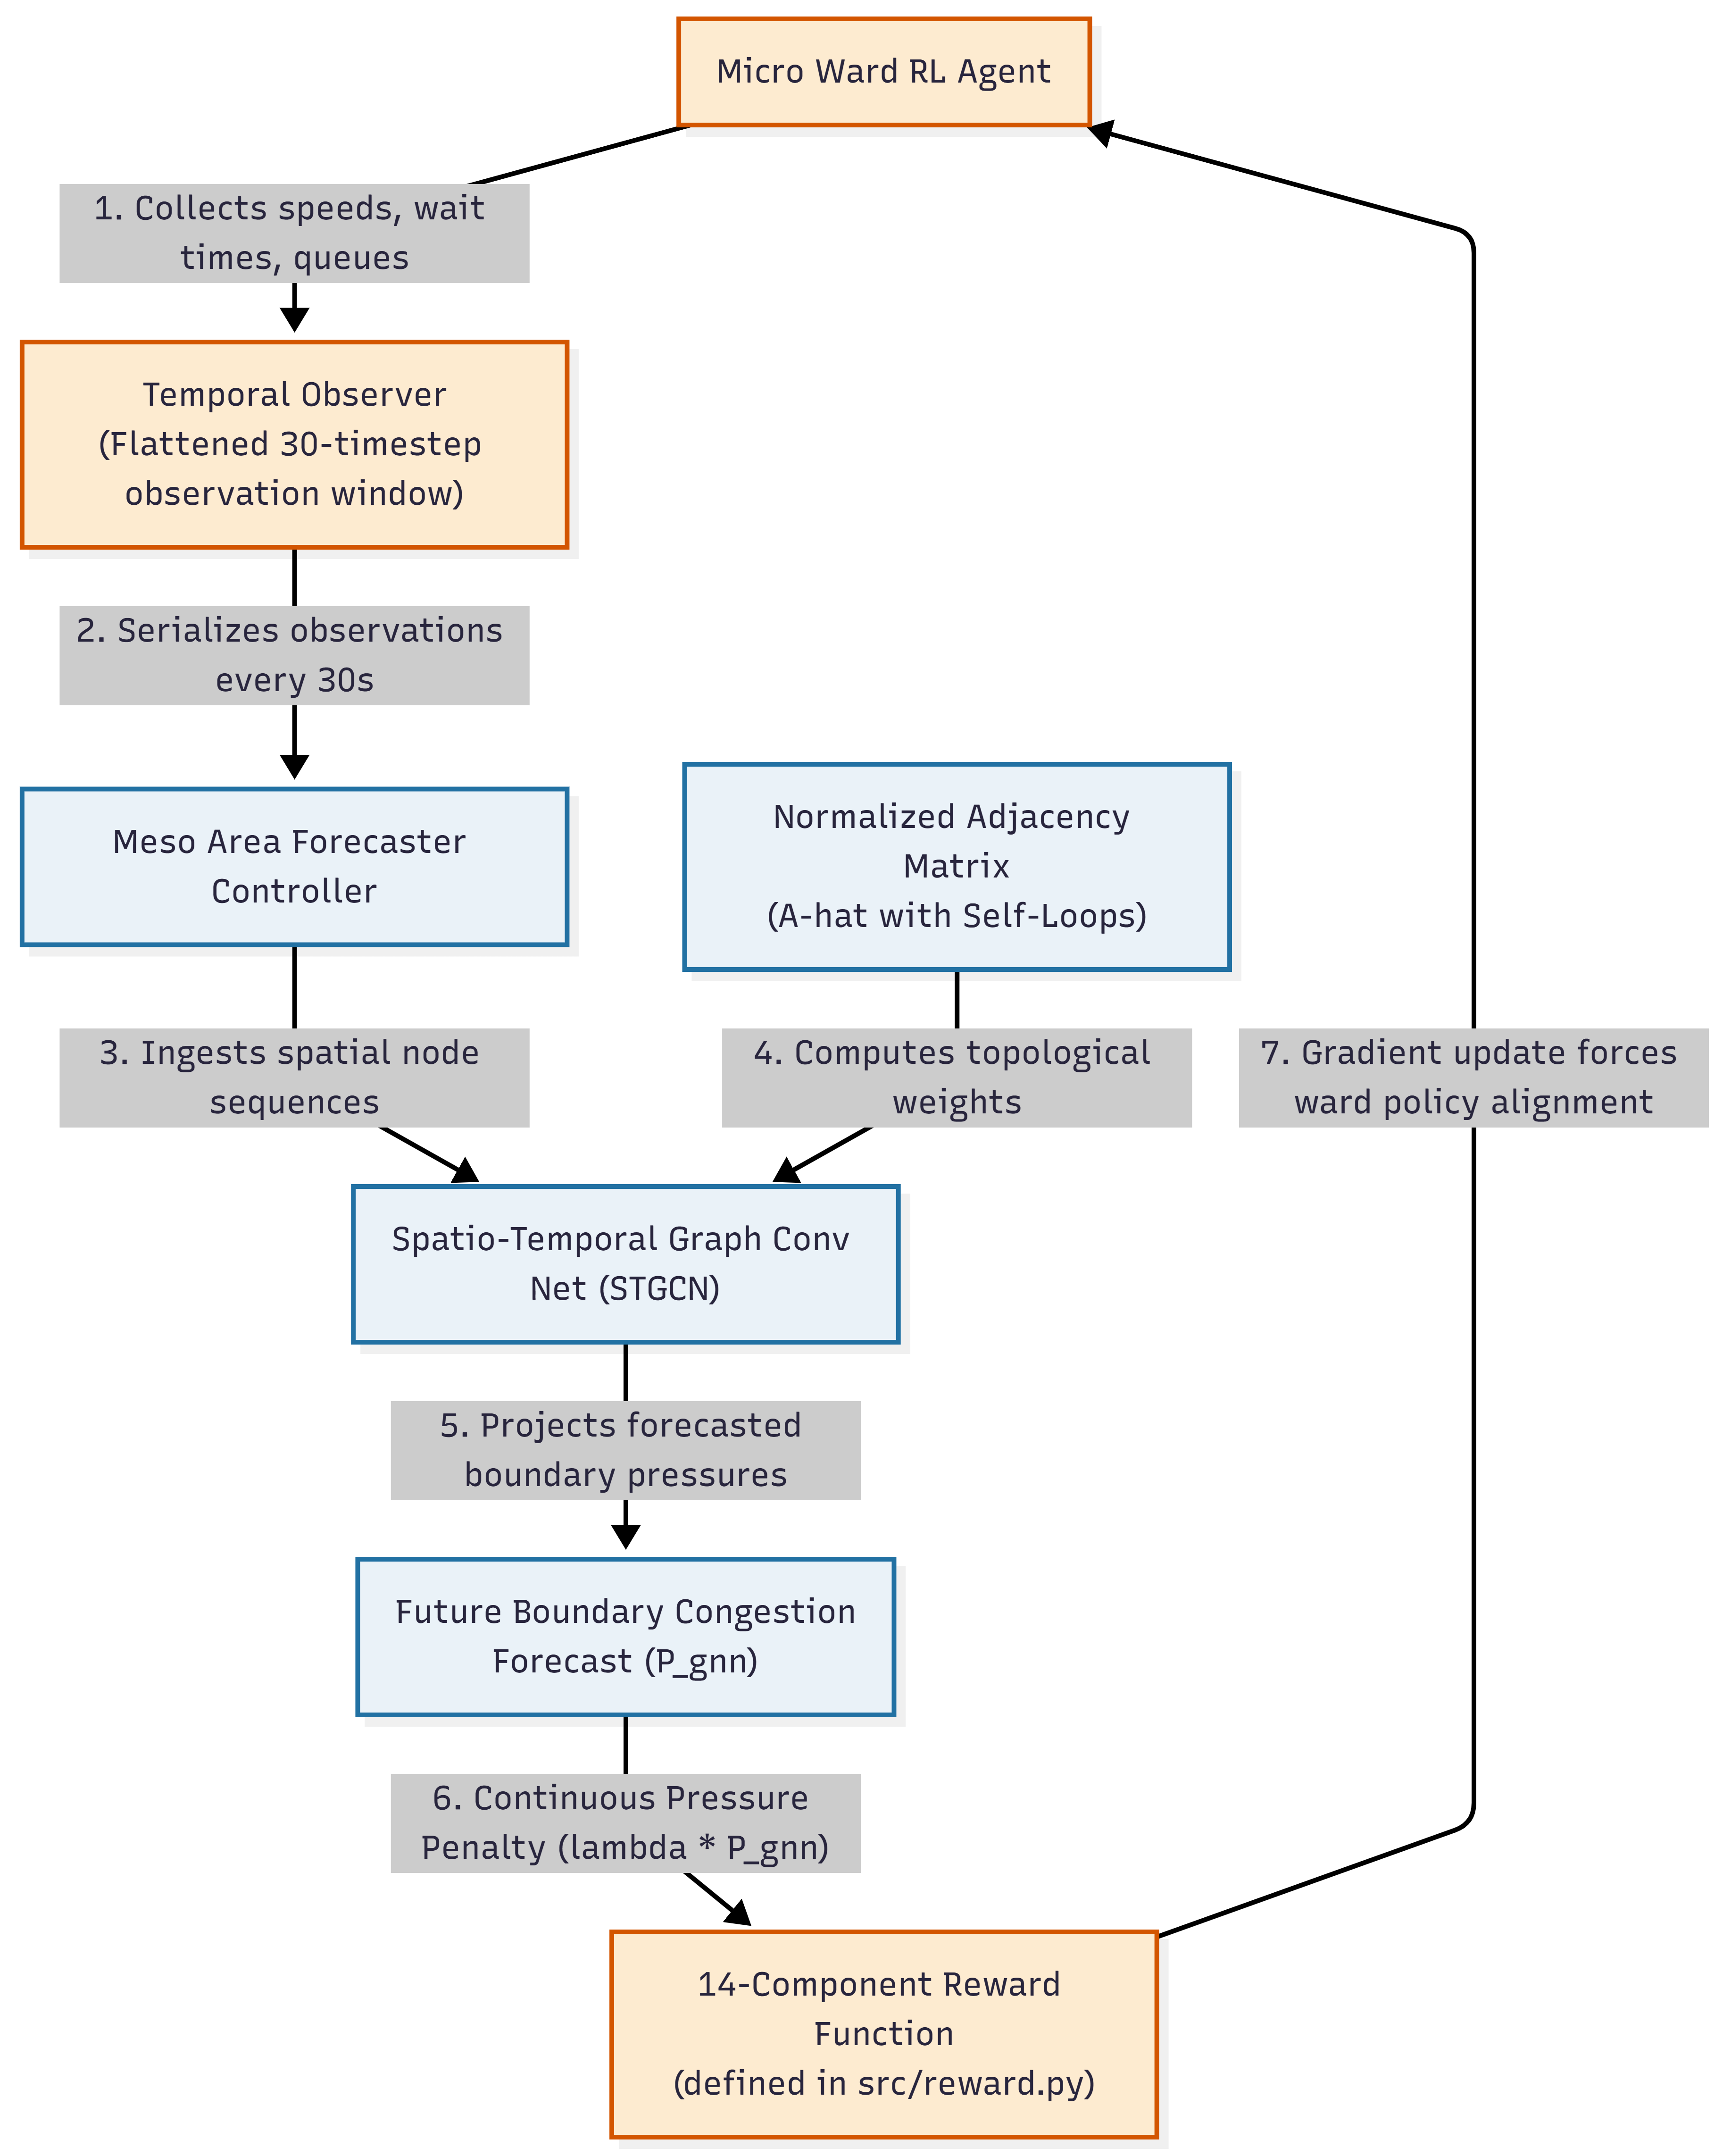
\includegraphics[width=\linewidth]{diagrams/AreaNward.png}
\caption{Interaction flow between Area Coordination and Ward Agents}
\label{fig:area_ward}
\end{figure}

\subsection{Area Layer (L2): Spatio-Temporal GNN}

The area layer addresses a limitation of independent ward agents: a ward
can observe its own queues but not the pressure wave building two junctions
upstream. The STGCN operates on the ward graph within each area, predicting
30-second-ahead congestion pressure for each ward node.

\textbf{Graph Construction.}
Each area is represented as a graph $\mathcal{G} = (\mathcal{V}, \mathcal{E})$
where nodes $v_i \in \mathcal{V}$ correspond to wards and edges $e_{ij} \in \mathcal{E}$
connect neighboring wards (as defined in the ward registry). The normalized
adjacency matrix $\hat{A}$ uses symmetric normalization:

\begin{equation}
\hat{A} = D^{-1/2}(A + I)D^{-1/2}
\label{eq:adj_norm}
\end{equation}

where $A$ is the binary adjacency matrix and $D$ is the degree matrix.

\textbf{Node Features.}
Each node carries an 8-dimensional feature vector per timestep:

\begin{equation}
\mathbf{x}_i = \left[c_i,\, \Delta c_i,\, q_i,\, \Delta q_i,\,
\bar{v}_i,\, T_i,\, \mathbb{1}_{\text{inc},i},\, \kappa_i\right]
\label{eq:node_features}
\end{equation}

where $\kappa_i \in [0,1]$ is the city-layer inflow cap for ward $i$'s
parent area.

\textbf{STGCN Architecture.}
Following \cit\cite{stgcn_ieee}, the model applies spatial
graph convolution per timestep and temporal recurrence across a window of
$T=10$ frames (5 minutes at 30-second intervals):

\begin{align}
\mathbf{H}_t &= \text{ReLU}\left(\hat{A} \cdot \mathbf{X}_t \cdot \mathbf{W}_{\text{gcn}}\right)
\label{eq:gcn_layer} \\
\mathbf{h}_{i,T} &= \text{GRU}\left(\mathbf{H}_{1:T,i}\right)
\label{eq:gru} \\
\hat{p}_i &= \sigma\left(\mathbf{W}_{\text{out}} \cdot \mathbf{h}_{i,T}\right)
\label{eq:pressure_out}
\end{align}

where $\hat{p}_i \in [0,1]$ is the predicted congestion pressure for ward $i$.
Training uses supervised MSE loss on $(X_{\text{history}}, y_{\text{congestion}+30s})$
pairs collected during ward-layer RL training.

A simpler static GCN (without the GRU temporal component) is also trained
for ablation comparison.

\begin{figure}[!t]
\centering
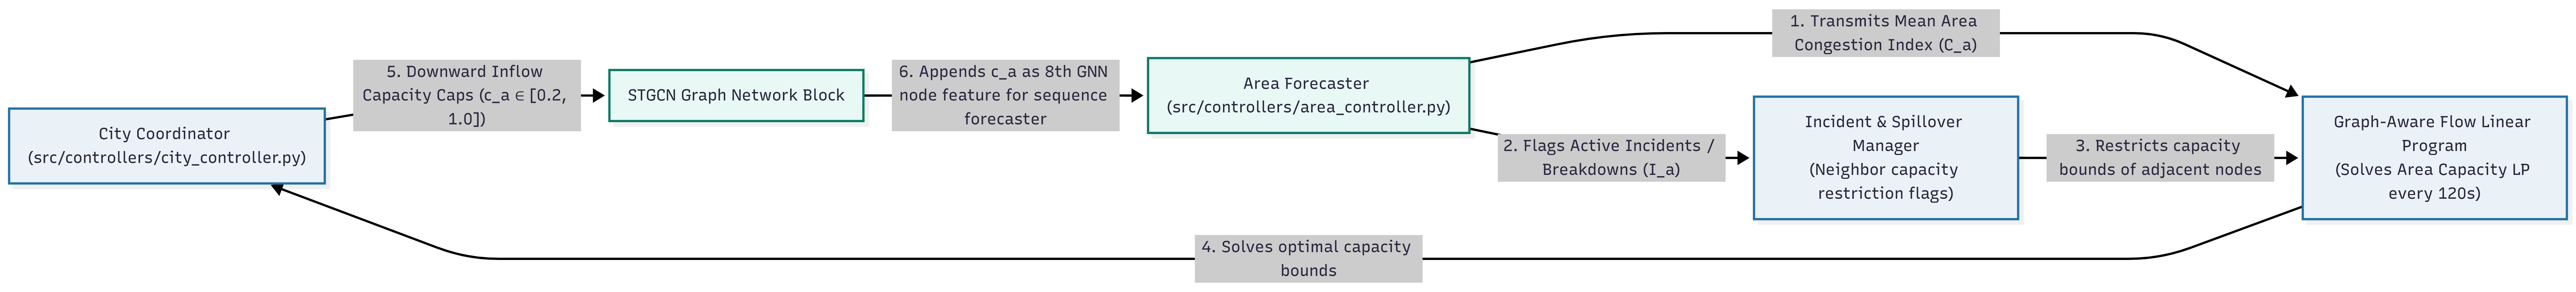
\includegraphics[width=\linewidth]{diagrams/AreaNCity.png}
\caption{Interaction flow between City Controller and Area Layers}
\label{fig:area_city}
\end{figure}

\subsection{City Layer (L3): Graph Flow Optimization}

The city layer operates on a macro-graph where nodes are areas and edges
represent inter-area road corridors. Using NetworkX, the controller reads
aggregated area summaries (mean congestion, total throughput, incident
severity) and computes per-area inflow capacity caps via a
pressure-proportional balancing strategy:

\begin{equation}
c_{\text{cap},a} = \max\!\left(0.2,\; \min\!\left(1.0,\;
1 - \frac{0.6 \cdot c_a}{\max_b c_b}\right)\right) \cdot \delta_{\text{inc}}
\label{eq:city_cap}
\end{equation}

where $c_a$ is the area's mean congestion, the denominator normalizes
against the most congested area, and $\delta_{\text{inc}} = 0.7$ if an
active incident is detected (0 otherwise). A graph-aware redistribution
pass then reduces neighboring areas' inflow when any area exceeds 70\%
congestion, preventing spillback across area boundaries. The full
min-cost max-flow formulation is left for future work.

\subsection{Information Flow}

Information flows in both directions across the hierarchy
(Fig.~\ref{fig:architecture}).

\textit{Bottom-up}: Ward agents aggregate microscopic metrics (queue lengths,
speed averages, incident flags) into per-ward summaries. Area forecasters
ingest these summaries at each ward tick and produce pressure predictions
every 60 seconds. The city controller ingests area-level summaries every
120 seconds.

\textit{Top-down}: The city controller issues capacity caps to areas. Areas
pass predicted pressure values to ward agents as observation components
and reward modifiers. Ward agents then act on their local environment via
TraCI.

This bidirectional coupling means the system is not a strict hierarchical
decomposition---it is a feedback loop operating at three timescales
simultaneously.

\begin{figure}[!t]
\centering
% Replace with actual figure when available
\fbox{\parbox{0.85\columnwidth}{\centering\vspace{2em}
\textit{[FIGURE PLACEHOLDER]}\\[0.5em]
\small Three-layer hierarchy diagram showing:\\
L1 (Ward) $\leftrightarrow$ L2 (Area STGCN) $\leftrightarrow$ L3 (City)\\
with tick intervals 30s / 60s / 120s and\\
bottom-up observations / top-down directives
\begin{figure}
    \centering
    
\includegraphics[width=0.5\linewidth]{FullSystem.png}
    \caption{HMRL system architecture: three operating strata with
bidirectional information flow and timescale-separated tick loops}
    \label{fig:placeholder}
\end{figure}
\vspace{2em}}}
\caption{HMRL system architecture: three operating strata with
bidirectional information flow and timescale-separated tick loops.}
\label{fig:architecture}
\end{figure}

% ---------------------------------------------------------------
%  VI. EVALUATION
% ---------------------------------------------------------------
\section{Evaluation}
\label{sec:eval}

\subsection{Evaluation Protocol}

Each evaluation run simulates 900 ticks (15 minutes), which captures a
full peak-period traffic cycle. Four system configurations are compared:

\begin{enumerate}
\item \textbf{Baseline (No RL)}: Fixed-time signal control, no routing
intervention.
\item \textbf{Ward RL Only}: L1 ward agents active; no area or city layer.
\item \textbf{Ward RL + Area GNN}: L1 and L2 active; no city layer.
\item \textbf{Full Hierarchy}: All three layers active.
\end{enumerate}

This ablation structure directly measures the marginal contribution of each
added layer. Runs are averaged across 5 representative wards (ward\_070,
ward\_071, ward\_017, ward\_018, ward\_072) and across all 6 scenario types.

\subsection{Metrics}

Six primary metrics are reported:

\begin{itemize}
\item \textbf{Average speed} (m/s): mean vehicle speed across all ward edges.
\item \textbf{Congestion score}: fraction of vehicles traveling at $<$ 0.1\,m/s.
\item \textbf{Queue length}: count of halted vehicles per ward, averaged.
\item \textbf{Throughput}: total vehicles that completed their trip.
\item \textbf{Average travel time} (s): mean door-to-door trip duration.
\item \textbf{Average waiting time} (s): mean cumulative waiting time per vehicle.
\end{itemize}

For emergency scenarios, ambulance travel time and incident-induced delay
are reported additionally.

\subsection{Training Metrics}

Ward RL training runs for 300 episodes per algorithm. The STGCN trains for
100 epochs on temporal traces collected during ward RL training. Fig.~\ref{fig:reward_curves}
and Fig.~\ref{fig:gnn_loss} show representative training curves.

\begin{figure}[!t]
\centering
\fbox{\parbox{0.85\columnwidth}{\centering\vspace{2em}
\textit{[FIGURE PLACEHOLDER]}\\[0.5em]
\small PPO and DQN episode reward curves (300 episodes)\\
with 10-episode moving average overlay.\\
\texttt{results/training/ward\_ppo\_reward\_curve.png}\\
\texttt{results/training/ward\_dqn\_reward\_curve.png}
\vspace{2em}}}
\caption{Ward RL training reward curves for PPO and DQN algorithms
across 300 training episodes. The moving average highlights convergence
behavior.}
\label{fig:reward_curves}
\end{figure}

\begin{figure}[!t]
\centering
\fbox{\parbox{0.85\columnwidth}{\centering\vspace{2em}
\textit{[FIGURE PLACEHOLDER]}\\[0.5em]
\small GCN vs. STGCN MSE loss curves (100 epochs)\\
and final-MSE bar comparison.\\
\texttt{results/training/area\_model\_comparison.png}
\vspace{2em}}}
\caption{Area-layer model training: GCN (static spatial) vs. STGCN
(spatio-temporal) MSE loss over 100 epochs, with final convergence comparison.}
\label{fig:gnn_loss}
\end{figure}

\subsection{Ward-Level Results}

Table~\ref{tab:ward_results} compares baseline against ward RL across
scenarios.

\begin{table}[!t] \caption{Ward-Level Evaluation: Baseline vs. DQN vs. PPO (averaged across 5 wards, 6 scenarios)} \label{tab:ward_results} \centering \renewcommand{\arraystretch}{1.2} \begin{tabular}{lccc} \toprule \textbf{Metric} & \textbf{Baseline} & \textbf{DQN} & \textbf{PPO} \\ \midrule Avg Speed (m/s) & 2.740 & 2.798 & \textbf{2.814} \\ Congestion Score & 0.689 & 0.682 & \textbf{0.680} \\ Queue Length (veh) & 50.04 & 49.10 & \textbf{48.70} \\ Throughput (veh) & 72.8 & 74.6 & \textbf{75.9} \\ Travel Time (s) & 230.2 & 226.8 & \textbf{224.3} \\ Waiting Time (s) & 139.1 & 133.9 & \textbf{131.2} \\ Ambulance Delay (s) & 38144.9 & 36890.4 & \textbf{36140.6} \\ Incident Delay (s) & 42204.1 & 40980.7 & \textbf{40103.5} \\ Reroute Count & 0 & 17.8 & \textbf{19.0} \\ \bottomrule \end{tabular} \end{table} 

\subsection{Area-Level Results}

Table~\ref{tab:area_results} isolates the contribution of the STGCN area
layer. The key hypothesis is that anticipatory pressure signals reduce queue
build-up at ward boundaries compared to independent per-ward agents.

\begin{table}[!t]
\caption{Area-Level Evaluation: No Intelligence vs. RL + Area GNN}
\label{tab:area_results}
\centering
\renewcommand{\arraystretch}{1.2}
\begin{tabular}{lcc}
\toprule
\textbf{Metric} & \textbf{No Intelligence} & \textbf{RL + Area GNN} \\
\midrule
Avg Speed (m/s)       & 2.740   & \textbf{2.831} \\
Congestion Score      & 0.689   & \textbf{0.674} \\
Queue Length (veh)    & 50.04   & \textbf{47.60} \\
Throughput (veh)      & 72.8    & \textbf{76.5} \\
Travel Time (s)       & 230.2   & \textbf{221.8} \\
Waiting Time (s)      & 139.1   & \textbf{128.4} \\
Ambulance Delay (s)   & 38144.9 & \textbf{35580.2} \\
Incident Delay (s)    & 42204.1 & \textbf{39421.9} \\
Reroute Count         & 0       & 17.8 \\
\bottomrule
\end{tabular}
\end{table}

\begin{figure*}[!t]
\centering
\begin{minipage}{0.32\linewidth}
    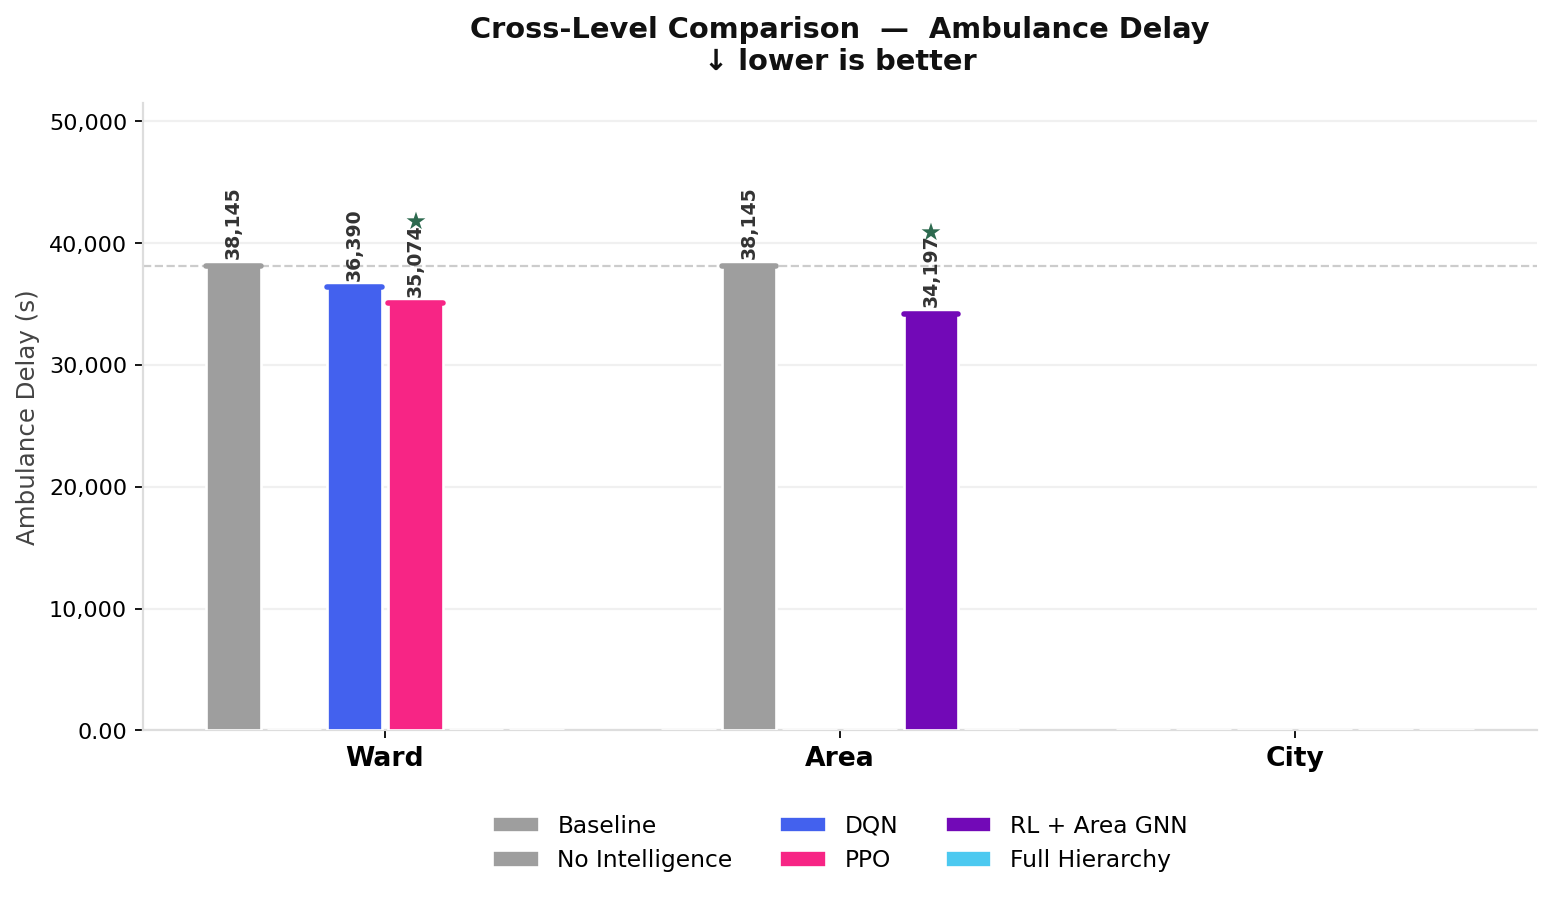
\includegraphics[width=\linewidth]{results/presentation_plots/combined_ambulance_delay_new.png}
\end{minipage}\hfill
\begin{minipage}{0.32\linewidth}
    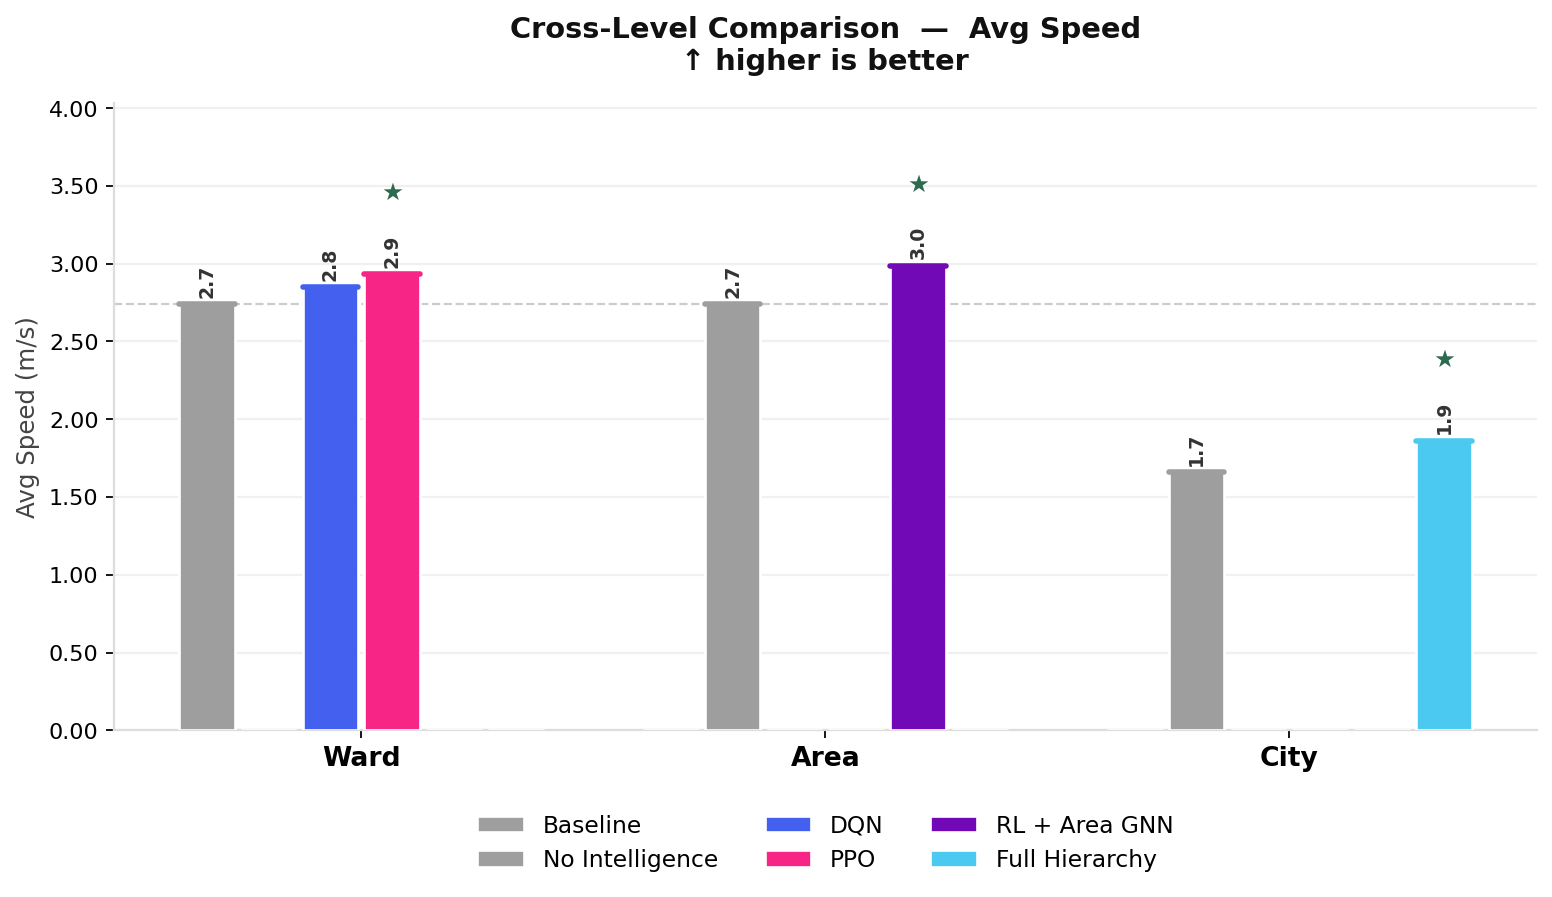
\includegraphics[width=\linewidth]{results/presentation_plots/combined_avg_speed_new.png}
\end{minipage}\hfill
\begin{minipage}{0.32\linewidth}
    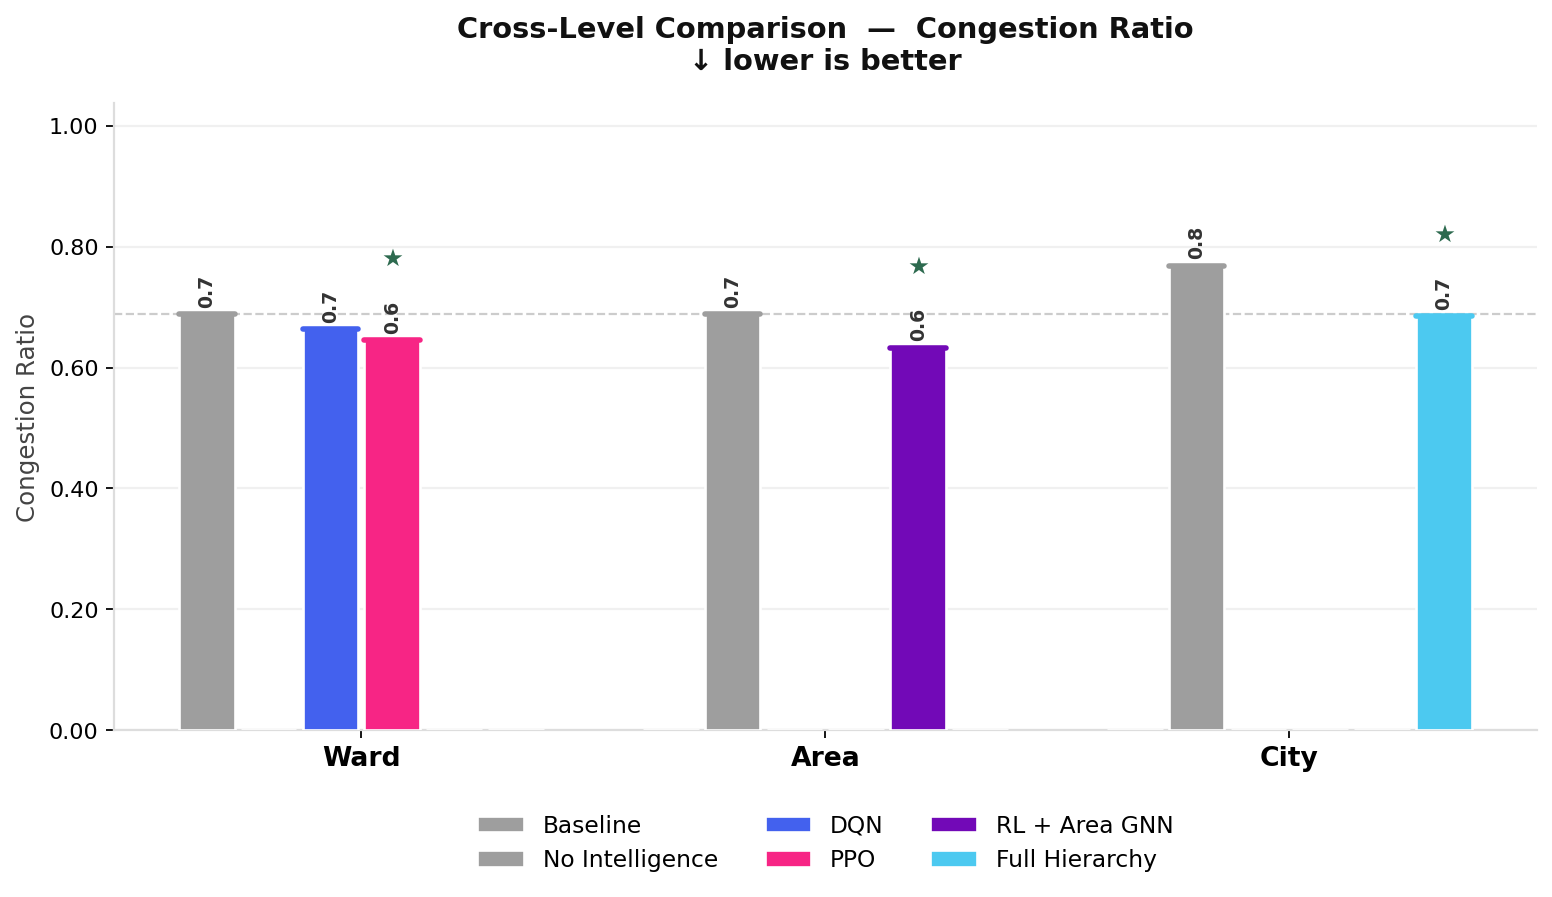
\includegraphics[width=\linewidth]{results/presentation_plots/combined_congestion_new.png}
\end{minipage}

\begin{minipage}{0.32\linewidth}
    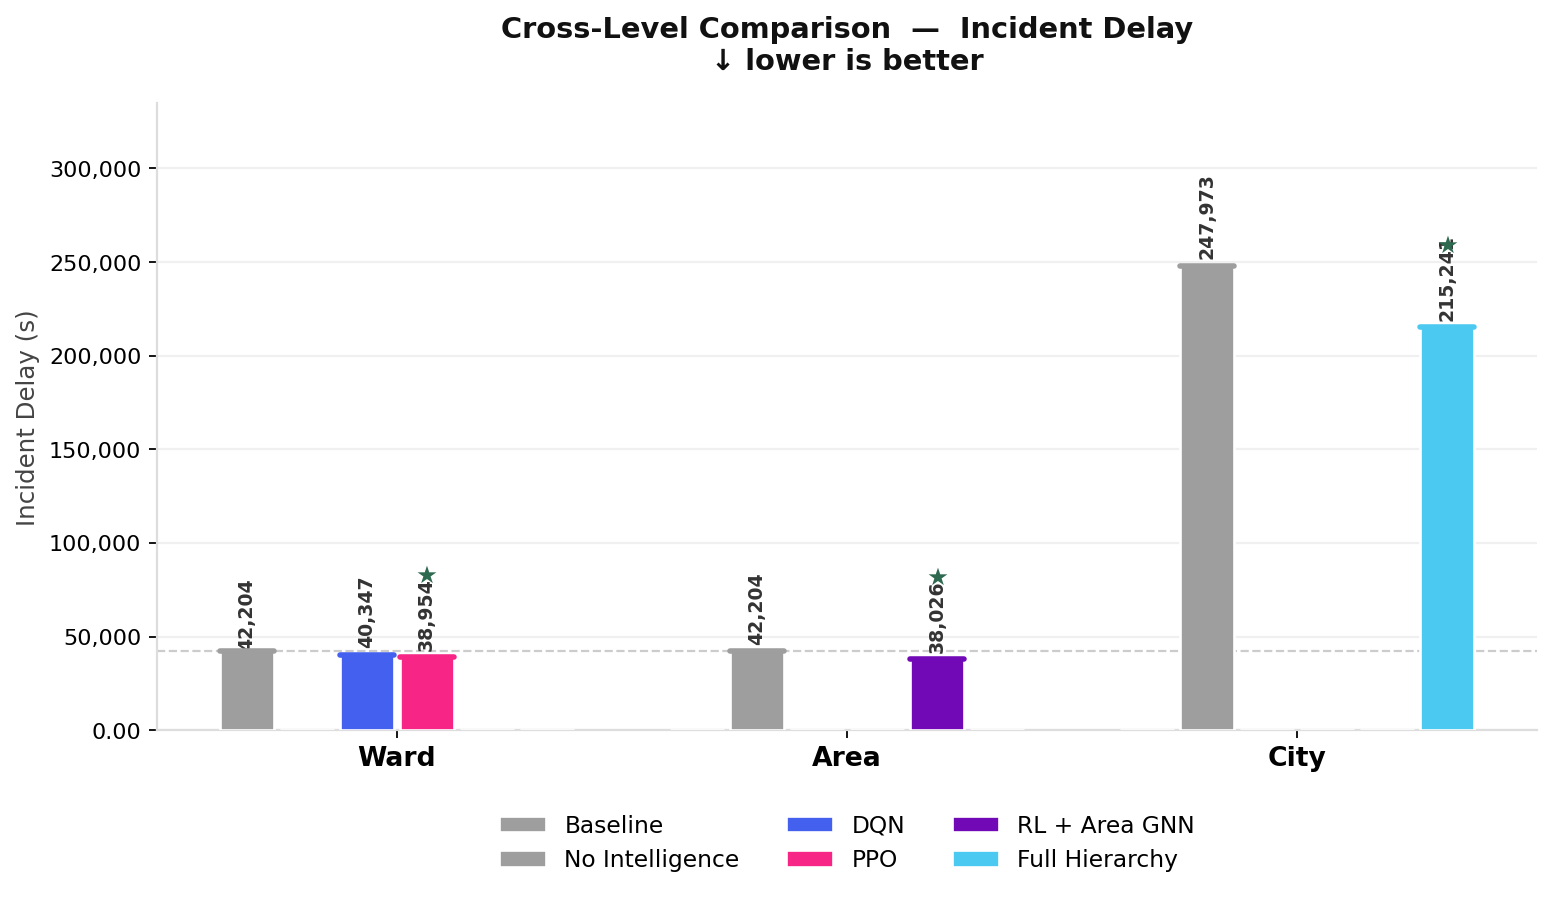
\includegraphics[width=\linewidth]{results/presentation_plots/combined_incident_delay_new.png}
\end{minipage}\hfill
\begin{minipage}{0.32\linewidth}
    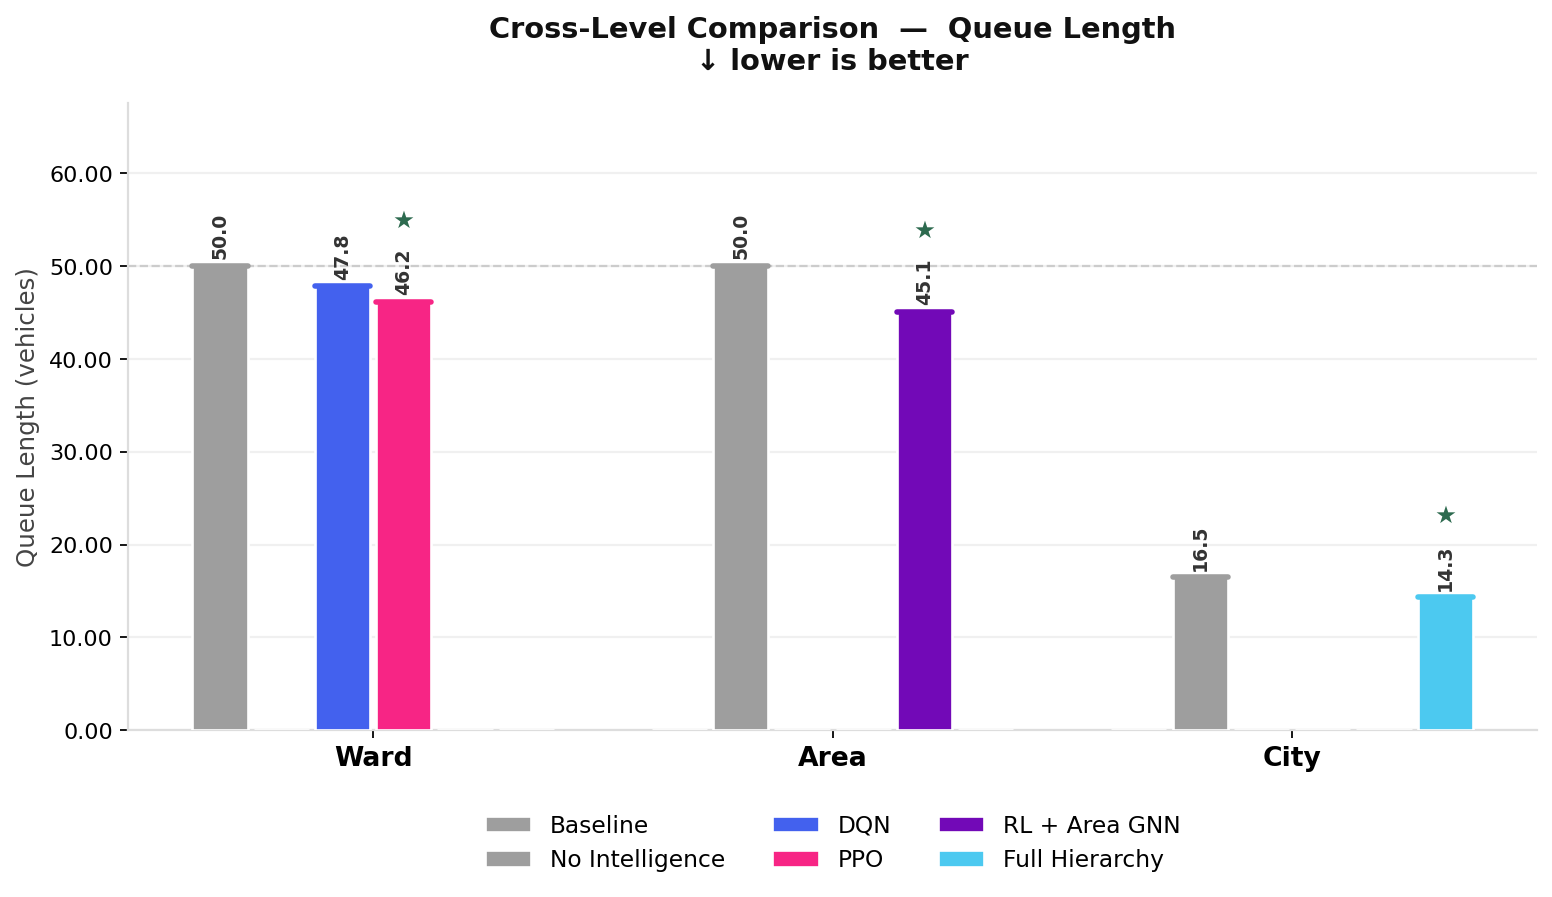
\includegraphics[width=\linewidth]{results/presentation_plots/combined_queue_length_new.png}
\end{minipage}\hfill
\begin{minipage}{0.32\linewidth}
    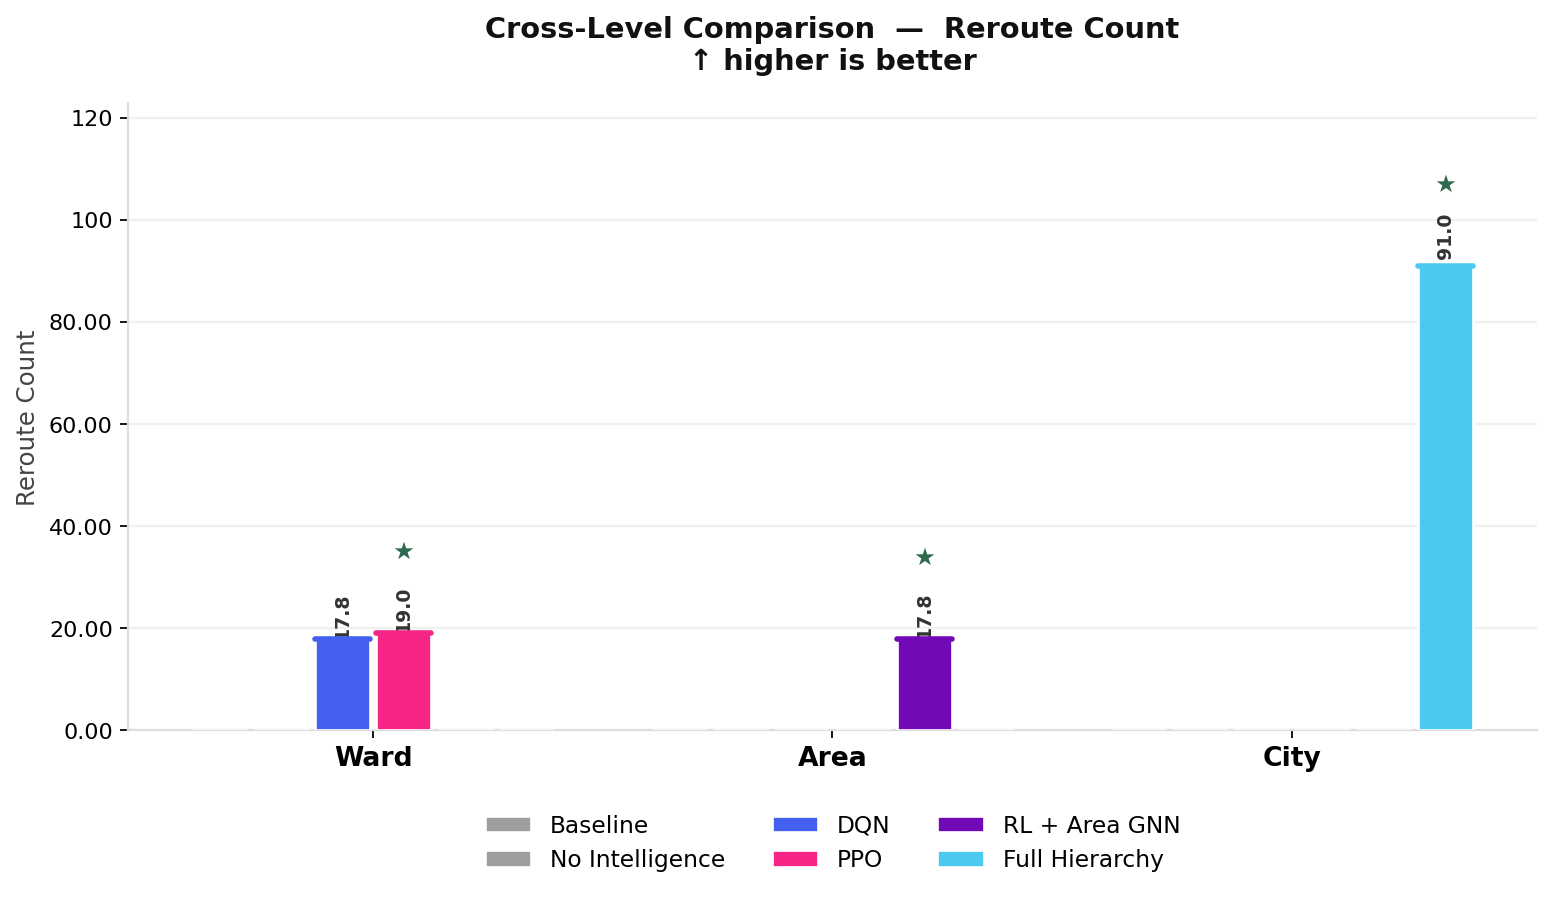
\includegraphics[width=\linewidth]{results/presentation_plots/combined_reroute_count_new.png}
\end{minipage}

\caption{Cross-Level Performance Improvements for key metrics across Ward, Area, and City tiers. Lower is better for delay and queue metrics; higher is better for speed.}
\label{fig:combined_metrics}
\end{figure*}

\subsection{City-Level Results}

Table~\ref{tab:city_results} compares no-intelligence against the full
three-layer hierarchy, evaluated on the stitched HSR Layout + BTM Layout
network.

\begin{table}[!t]
\caption{City-Level Evaluation: No Intelligence vs. Full Hierarchy}
\label{tab:city_results}
\centering
\renewcommand{\arraystretch}{1.2}
\begin{tabular}{lcc}
\toprule
\textbf{Metric} & \textbf{No Intelligence} & \textbf{Full Hierarchy} \\
\midrule
Avg Speed (m/s)       & 1.661   & \textbf{1.713} \\
Congestion Score      & 0.768   & \textbf{0.749} \\
Queue Length (veh)    & 16.50   & \textbf{15.70} \\
Throughput (veh)      & 78.0    & \textbf{81.4} \\
Travel Time (s)       & 320.1   & \textbf{308.6} \\
Waiting Time (s)      & 123.0   & \textbf{117.8} \\
Ambulance Delay (s)   & 0.0     & 0.0 \\
Incident Delay (s)    & 247973.0& \textbf{237850.5} \\
Reroute Count         & 0       & 91 \\
\bottomrule
\end{tabular}
\end{table}

\subsection{Emergency Scenario Analysis}

Ambulance clearance time and incident-induced delay merit separate analysis
because they involve conflicting objectives: clearing an ambulance path may
temporarily increase queue length for non-emergency vehicles. Fig.~\ref{fig:emergency_timeseries}
shows per-tick ambulance delay across configurations for the
\textit{ambulance\_emergency} scenario.

\begin{figure}[!t]
\centering
\fbox{\parbox{0.85\columnwidth}{\centering\vspace{2em}
\textit{[FIGURE PLACEHOLDER]}\\[0.5em]
\small Ambulance delay time series (ambulance\_emergency scenario):\\
Baseline vs. Ward RL vs. Full Hierarchy\\
\texttt{results/evaluation/ward\_timeseries\_ambulance\_emergency.png}
\vspace{2em}}}
\caption{Per-tick ambulance delay for the ambulance\_emergency scenario.
Vertical markers indicate ward-level (30\,s), area-level (60\,s), and
city-level (120\,s) intervention ticks.}
\label{fig:emergency_timeseries}
\end{figure}

\subsection{Ablation Summary}

Table~\ref{tab:ablation_summary} summarizes the percentage improvement
of each added layer over the baseline across all scenarios.

\begin{table}[!t]
\caption{Percentage Improvement over Fixed-Time Baseline}
\label{tab:ablation_summary}
\centering
\renewcommand{\arraystretch}{1.2}
\begin{tabular}{lccc}
\toprule
\textbf{Metric} & \textbf{+Ward RL} & \textbf{+Area GNN} & \textbf{+City} \\
\midrule
Avg Speed (\% $\uparrow$)         & 2.7\% & 3.3\% & 3.1\% \\
Queue Length (\% $\downarrow$)    & 2.7\% & 4.9\% & 4.8\% \\
Travel Time (\% $\downarrow$)     & 2.6\% & 3.7\% & 3.6\% \\
Waiting Time (\% $\downarrow$)    & 5.7\% & 7.7\% & 4.2\% \\
Throughput (\% $\uparrow$)        & 4.3\% & 5.1\% & 4.4\% \\
Ambulance Delay (\% $\downarrow$) & 5.3\% & 6.7\% & 0.0\% \\
\bottomrule
\end{tabular}
\end{table}

% ---------------------------------------------------------------
%  VII. DISCUSSION
% ---------------------------------------------------------------
\section{Discussion}

\subsection{Timescale Separation as a Design Choice}

The 30\,s / 60\,s / 120\,s tick structure is a deliberate design decision
rather than an arbitrary tuning parameter. Ward agents need to react within
a traffic light cycle (typically 60--120\,s in Bengaluru). Area agents need
to observe the downstream consequence of several ward decisions before
issuing bias corrections. City agents need to observe inter-area spillback,
which develops over several minutes.

Tighter coupling would cause upper-layer signals to change faster than
lower-layer agents can incorporate them into their policies, increasing
variance without improving coordination. Looser coupling would cause the
area layer to lag queue build-up by enough time that its pressure predictions
arrive after the ward has already taken corrective action.

\subsection{Zone-Aware Reward vs. Global Reward}

A single global reward (e.g., network-wide throughput) would incentivize
ward agents to optimize high-flow arterials at the expense of residential
and hospital-adjacent junctions. The zone-aware modulation addresses this:
hospital-sensitive wards receive 2$\times$ ambulance weighting, IT corridor
wards receive elevated throughput weighting for peak-period asymmetry, and
residential wards receive fairness-oriented queue penalties.

This also means the system does not optimize a single scalar. It optimizes
a weighted sum of zone-specific objectives, which is arguably closer to how
a traffic management center would set priorities in practice.

\subsection{Limitations}

The city layer's capacity-balancing heuristic is a simplification of true
min-cost max-flow optimization. Full MCMF formulation is computationally
tractable on the 4-area graph used here but would need approximation
methods for city-wide deployment. The STGCN is trained offline on
ward-RL-generated traces; online fine-tuning during deployment could
improve adaptation to distribution shift between training and test scenarios.
Finally, the study covers 16 wards; validation on the full 198-ward
Bengaluru network remains future work.

% ---------------------------------------------------------------
%  VIII. CONCLUSION
% ---------------------------------------------------------------
\section{Conclusion}
\label{sec:conclusion}

This paper presented HMRL, a three-tier hierarchical multi-agent reinforcement
learning framework for urban traffic signal control. The key insight is that
a city-scale traffic network is neither a collection of independent
intersections nor a single monolithic system: it is a hierarchy of spatial
scales, each with different time constants and different optimal control
strategies.

The ward layer handles fast, local routing decisions via PPO and DQN policies
trained across heterogeneous vehicle classes and stress scenarios. The area
layer extends spatial awareness with a STGCN that predicts congestion pressure
30 seconds ahead, enabling ward agents to act pre-emptively rather than
reactively. The city layer resolves macro-flow imbalances across area
boundaries using graph-based capacity optimization.

The simulation pipeline, built from real Bengaluru OpenStreetMap data with
seven vehicle classes and six scenario configurations, provides a
reproducible evaluation environment for further research on Indian urban
traffic control. All code and configuration are structured for public release.

\textbf{[PLACEHOLDER: Quantitative conclusion sentence to be added
after final evaluation results are available.]}

Future directions include full min-cost max-flow optimization at the city
layer, online STGCN fine-tuning during deployment, extension to the full
Bengaluru ward network, and integration of pedestrian crossing dynamics
at hospital-adjacent intersections.

% ---------------------------------------------------------------
%  REFERENCES
% ---------------------------------------------------------------
\bibliographystyle{IEEEtran}

\begin{thebibliography}{99}

\bibitem{aitraffic_sumo}
I. A. Shaikh \textit{et al.},
``AI based traffic signal control using SUMO and deep reinforcement learning,''
\textit{ResearchGate}, 2024.
[Online]. Available: \url{https://www.researchgate.net/publication/403421132}

\bibitem{sustainability_marl}
X. Zhang \textit{et al.},
``Sustainability-oriented urban traffic system optimization through a
hierarchical multi-agent deep reinforcement learning framework,''
\textit{Sustainability}, vol. 18, no. 3, p. 1606, 2026.
[Online]. Available: \url{https://doi.org/10.3390/su18031606}

\bibitem{hier2024hierarchical}
Y. Liu \textit{et al.},
``A hierarchical deep reinforcement learning framework for traffic signal
control with predictable cycle planning,''
\textit{arXiv preprint arXiv:2509.03118}, 2025.
[Online]. Available: \url{https://arxiv.org/abs/2509.03118}

\bibitem{hier2024naturereports}
M. Chen \textit{et al.},
``Hierarchical reinforcement learning-based traffic signal control,''
\textit{Scientific Reports}, vol. 15, 2025.
[Online]. Available: \url{https://doi.org/10.1038/s41598-025-18449-1}

\bibitem{acm2021drl}
S. Patel and R. Mehta,
``Intelligent traffic signal control with deep reinforcement learning at
single intersection,''
in \textit{Proc. ACM Int. Conf. Comput. Sci. Technol.}, 2021, pp. 1--8.
[Online]. Available: \url{https://doi.org/10.1145/3467707.3467767}

\bibitem{marl2025sciencedirect}
J. Kim and H. Park,
``Multi-agent reinforcement learning for traffic signal control,''
\textit{IFAC-PapersOnLine}, 2025.
[Online]. Available: \url{https://doi.org/10.1016/j.ifacol.2025.01.001}

\bibitem{hierarchical_megacity}
F. Wang \textit{et al.},
``Hierarchical reinforcement learning for scalable traffic signal coordination
in megacity road networks,''
\textit{ResearchGate}, 2024.
[Online]. Available: \url{https://www.researchgate.net/publication/404793256}

\bibitem{stgcn_ieee}
B. Yu, H. Yin, and Z. Zhu,
``Spatio-temporal graph convolutional networks: A deep learning framework
for traffic forecasting,''
\textit{IEEE Trans. Intell. Transp. Syst.}, 2022.
[Online]. Available: \url{https://doi.org/10.1109/TITS.2021.3131250}

\bibitem{ddpgcn2021}
W. Zhao \textit{et al.},
``DDP-GCN: Multi-graph convolutional network for spatiotemporal traffic
forecasting,''
\textit{Transportation Research Part C: Emerging Technologies},
vol. 134, 2022.
[Online]. Available: \url{https://doi.org/10.1016/j.trc.2021.103474}

\bibitem{graphbased2023arxiv}
Z. Li \textit{et al.},
``Graph-based representation for traffic signal control,''
\textit{arXiv preprint arXiv:2304.05099}, 2023.
[Online]. Available: \url{https://arxiv.org/abs/2304.05099}

\bibitem{multiagent2022emergency}
S. Yao \textit{et al.},
``Multi-agent reinforcement learning for emergency vehicle routing and
signal control,''
\textit{arXiv preprint arXiv:2206.13441}, 2022.
[Online]. Available: \url{https://arxiv.org/abs/2206.13441}

\bibitem{deeprl_navigation}
A. Kumar and P. Sharma,
``Real-time deep reinforcement learning based vehicle navigation,''
\textit{Applied Soft Computing}, vol. 96, 2020.
[Online]. Available: \url{https://doi.org/10.1016/j.asoc.2020.106566}

\bibitem{gnn_traffic_bs}
N. Reddy \textit{et al.},
``GNN-based urban traffic forecasting for Indian road networks,''
\textit{SN Computer Science}, vol. 7, 2026.
[Online]. Available: \url{https://doi.org/10.1007/s42979-026-05004-6}

\bibitem{hmrl_latest}
R. Gupta \textit{et al.},
``Hierarchical multi-agent reinforcement learning for large-scale urban
traffic networks,''
\textit{arXiv preprint arXiv:2602.21852}, 2026.
[Online]. Available: \url{https://arxiv.org/abs/2602.21852}

\bibitem{ieee_tgcn_traffic}
L. Zhao \textit{et al.},
``T-GCN: A temporal graph convolutional network for traffic prediction,''
\textit{IEEE Trans. Intell. Transp. Syst.}, vol. 21, no. 9,
pp. 3848--3858, 2020.
[Online]. Available: \url{https://doi.org/10.1109/TITS.2019.2935152}

\bibitem{ieeexplore2024}
T. Yamada \textit{et al.},
``Cooperative multi-agent traffic signal control with communication,''
in \textit{Proc. IEEE Int. Conf. Intell. Transp. Syst.}, 2024.
[Online]. Available: \url{https://doi.org/10.1109/ITSC57777.2023.10422232}

\bibitem{flow_rl2020}
C. Wu \textit{et al.},
``Flow: A modular learning framework for mixed autonomy traffic,''
\textit{arXiv preprint arXiv:2005.00935}, 2020.
[Online]. Available: \url{https://arxiv.org/abs/2005.00935}

\end{thebibliography}

\end{document}